\documentclass[a4paper,11pt]{article}

\usepackage[T1]{fontenc}
\usepackage[utf8]{inputenc}
\usepackage[english]{babel}
\usepackage[top=3cm, left=2cm, textwidth=17cm, textheight=24cm]{geometry}
\usepackage{times}
\usepackage{multirow}
\usepackage[ruled, czech, linesnumbered, noline, longend]{algorithm2e}
\usepackage{graphics}
\usepackage{pdflscape}
\usepackage{float}
\usepackage{tabularx}
\usepackage{array}


\usepackage[unicode, hidelinks]{hyperref}
\usepackage[nodayofweek]{datetime}
\usepackage[hyphenbreaks]{breakurl}
\usepackage{csquotes}
 
\begin{document}

\begin{titlepage}
    \begin{center}
        
        \Huge
        \textsc{Vysoké učení technické v~Brně}\\[0.1em]
        
        \huge
        \textsc{Fakulta~informačních technologií}
        
        \vspace*{\stretch{0.382}}
        
        \LARGE
        IMAP Client --\ Manual \\[-0.1em]

        \vspace*{\stretch{0.618}}
    \end{center}
    
    {\Large \today \hfill Tomáš Dolák}
\end{titlepage}

\newpage
\tableofcontents

\newpage
\label{firstpage}
\section{Introduction}
The project assignment in the ISA (Network Applications and Network Administration) subject was 
to create IMAP4rev1 (according to RFC3501), which will be able to communicate only over TCP/IP as well 
as using SLL/TLS - IMAPS. The following program downloads emails from the defined server in the argument 
of the program call and saves them in the output directory. If the path to the output repository 
specified by the argument does not exist, the program creates it on this path.

\subsection{IMAP in Email Services and How It's Used}

\subsubsection{Internet Message Access Protocol}
The Internet Message Access Protocol (IMAP) is a protocol for receiving email that allows users to access 
their mailboxes from any device with an internet connection. IMAP was designed to provide flexibility in 
accessing email messages, regardless of the device or application used. This is achieved by acting as an 
intermediary between the email server and client, rather than directly downloading emails onto the device. 
However, IMAP also allows emails to be stored locally, a feature leveraged by this program to download 
and store emails on the user’s device \cite{rfc3501, what_is_imap}.

While IMAP enhances flexibility, it does come with security considerations. By default, IMAP transmits 
login credentials in plain text, leaving usernames and passwords vulnerable if intercepted. This issue 
can be mitigated by configuring IMAP to operate over Transport Layer Security (TLS), which can be enabled 
in our program using the \texttt{-T} parameter, encrypting the communication between the client and server. 
Using TLS is a recommended practice to improve IMAP security \cite{what_is_imap, imap_pop_difference, email_protocols}.

\subsubsection{How IMAP Works?}
IMAP establishes a connection between the email client and server. In most email applications, IMAP allows users to view email headers quickly and download full messages only when selected, which conserves data. Outgoing emails, on the other hand, are sent via the Simple Mail Transfer Protocol (SMTP), which handles message delivery to the recipient \cite{techtarget_imap, email_protocols}.


\section{Using the \texttt{imapcl} Program}
The \texttt{imapcl} program is designed to download email messages from a server via IMAP protocol, 
with optional support for encrypted connections via SSL/TLS. To run the program, use the following 
command syntax:

\begin{verbatim}
    imapcl server [-p port] [-T [-c certfile] [-C certaddr]] [-n] [-h] \
    -a auth_file [-b MAILBOX] -o out_dir
\end{verbatim}

The order of parameters is flexible. Below is a description of each parameter:

\subsection{Required Parameters}
\begin{itemize}
    \item \texttt{server}: IP address or domain name of the IMAP server.
    \item \texttt{-a auth\_file}: Path to the file containing user authentication credentials.
    \item \texttt{-o out\_dir}: Output directory where downloaded messages will be saved.
\end{itemize}

\subsection{Optional Parameters}
\begin{itemize}
    \item \texttt{-p port}: Specifies the server port. The default value depends on whether the \texttt{-T} parameter is used (use port 993 for encrypted connections).
    \item \texttt{-T}: Enables an encrypted connection using the IMAPS protocol. If not specified, an unencrypted connection (port 143) is used.
    \item \texttt{-c certfile}: Path to a certificate file used to verify the validity of the server’s SSL/TLS certificate.
    \item \texttt{-C certaddr}: Path to a directory containing certificates to verify the SSL/TLS certificate presented by the server. The default value is \texttt{/etc/ssl/certs}.
    \item \texttt{-n}: Only new messages – the program will work only with messages that have not yet been downloaded.
    \item \texttt{-h}: Download only message headers without the content.
    \item \texttt{-b MAILBOX}: Specifies the mailbox name on the server. The default is \texttt{INBOX}.
\end{itemize}

Example how to use the program:

\begin{verbatim}
./imapcl imap.outlook.cz -p 143 -a ~/Desktop/auth_file.txt -b INBOX \
-o ~/Desktop/email/user_inbox/
\end{verbatim}

If program is called wrongly or with wrong arguments, the program will print a help message to the user.

\subsection{Examples of Downloaded Email Filenames}
If the arguments \texttt{-h} and \texttt{-n} are not used, the output filenames of downloaded emails will look like this:
\begin{verbatim}
MSG_INBOX_1717.txt
\end{verbatim}
where \texttt{INBOX} is the mailbox and \texttt{1717} is the UID of this email.

If the arguments \texttt{-h} and \texttt{-n} are used, the output filenames of downloaded emails will look like this:
\begin{verbatim}
MSG_INBOX_1717_new_header.txt
\end{verbatim}
where \texttt{INBOX} is the mailbox, \texttt{1717} is the UID of this email, and \texttt{new\_header} indicates that the email contains just the header of emails that the IMAP server categorizes as new.

If only the argument \texttt{-h} is used, the output filenames of downloaded emails will look like this:
\begin{verbatim}
MSG_INBOX_1717_header.txt
\end{verbatim}
where \texttt{INBOX} is the mailbox, \texttt{1717} is the UID of this email, and \texttt{header} indicates that the file contains only the email's header.

If only the argument \texttt{-n} is used, the output filenames of downloaded emails will look like this:
\begin{verbatim}
MSG_INBOX_1717_new.txt
\end{verbatim}
where \texttt{INBOX} is the mailbox, \texttt{1717} is the UID of this email, and \texttt{new} indicates that the file contains an email that the IMAP server categorizes as new.


\section{Implementation Details}
The principles of object-oriented programming have been applied to the program code. The program is 
divided into logical classes such as the \verb!ClientConfig! class - which takes care of the configuration 
of the resulting IMAP client based on the input arguments of the program, which it also processes. 
On the result of the configuration, either an instance of the \verb!NonSecureImapClient! class is created, 
which mediates communication, classically only over TCP/IP, or an instance of the \verb!SecureImapClient! 
class, which also uses SSL/TLS in addition to TCP/IP. Both classes \verb!NonSecureImapClient! and 
\verb!SecureImapClient! inherit basic properties from \verb!BaseImapClient!, which provides features 
that are common to both derived classes, such as generating a TAG, finding the value of the current TAG or translating 
a hostname to an IPv4 address.\cite{openssl_tutorial}

\subsection{Implementation of Client}
The NonSecureImapClient and SecureClient classes are characterized by their very 
similar behavior, at the beginning when the class is instantiated they receive information 
like \verb!MailBox!, \verb!OutputDirectory!, \\ 
\verb!HeadersOnly! and \verb!NewOnly! as input parameters. These parameters are used to define 
further behavior of the program and their description is given in table below.

\smallskip

\begin{center}
    \vspace{0.5cm} % Space before table
    \begin{tabular}{|c|c|}
        \hline
        \textbf{Parameter} & \textbf{Description} \\
        \hline
        MailBox & Mailbox from which emails will be downloaded \\
        \hline
        OutputDirectory & Specifies where downloaded emails will be stored \\
        \hline
        HeadersOnly & Only header of the emails will be downloaded \\
        \hline
        NewOnly & Only unseen emails will be downloaded \\
        \hline
    \end{tabular}
    \vspace{0.5cm} % Space after table
\end{center}

Then, from the user's point of view, the classes only need to call the Run method with the parameters 
server address, port login and password. This method interacts with the server and its behaviour is as follows.

\subsection{Program's Features}

\subsubsection{Usage of UIDVALIDITY Value}
The program also contains some of the extra features, the first of which is that the client 
saves a special \verb!.uidvalidity! file with the value \verb!UIDVALIDITY! when downloading 
to a specific output directory for the first time, this value is used in case the user wants 
to repeatedly download files to the same \verb!output! \verb!directory! and have synchronized mailboxes. 
On each subsequent run, the \verb!UIDVALIDITY! value is checked to see if it is the same locally 
(in this \verb!.uidvalidity! file) and on the server, if the values are different, 
it is a sign that the structure of the mailbox on the server has changed (i.e. the emails 
have been removed or moved to another mailbox, etc.) and the output directory needs to be purged 
and the emails downloaded again. 
The \verb!.uidvalidity! file is formatted according to the rule that each \verb!mailbox! has its 
corresponding line, which contains the mailbox name followed by the equal and finally the 
\verb!uidvalidity value! for the given mailbox. Note that the file is not associated with the 
name of the IMAP server or user account, so it is recommended to download only emails from 
multiple mailboxes of one account to one output directory to maintain clarity and easy orientation 
in the application output.

An example of the `.uidvalidity` file content:

\begin{verbatim}
INBOX=1662988148
SPECIFIC_MAILBOX1=1662988155
SPECIFIC_MAILBOX2=1362922155
\end{verbatim}

\newpage

In this example:
\begin{itemize}
    \item \texttt{INBOX=1662988148} indicates that the \texttt{uidvalidity} value for the "INBOX" mailbox is\\ \texttt{1662988148}.
    \item \texttt{SPECIFIC\_MAILBOX1=1662988155} indicates that the \texttt{uidvalidity} value\\ 
    for the "SPECIFIC\_MAILBOX1" mailbox is \texttt{1662988155}.
    \item \texttt{SPECIFIC\_MAILBOX2=1362922155} indicates that the \texttt{uidvalidity} value\\
     for the "SPECIFIC\_MAILBOX2" mailbox is \texttt{1362922155}.
\end{itemize}

This is done to ensure that the locally downloaded emails are always synchronized with those 
on the server and to allow users to download emails from multiple mailboxes to a single output 
directory. 

\subsubsection{Creation of Output Directory}
The client always needs to have a specific \verb!output directory! to which it will download emails 
from the IMAP server, it can happen that the user specifies his/her own location, but the 
folder on the given path does not exist (for example \verb!-o /Desktop/email/my_mailbox/!) in 
this case the client is able to create the folder on the given path 
(in this example on \verb!/Desktop/email/my_mailbox/!) and store the emails in it.

\subsubsection{Store Emails From Multiple Mailboxes Into One Output Directory}
The user of \verb!imapcl! has the possibility to download emails from several mailboxes 
into one \verb!output! directory, the names of output files with saved emails are defined 
according to the \verb!UID value! of the given email and according to the \verb!mailbox! 
to which the email is saved. it is highly recommended not to mix emails e.g. from two IMAP 
servers into one output directory, in case of a mailbox name match the emails from the previous 
download will be deleted and replaced by the current download.

\subsubsection{Gentle Download}
The program also introduces a \textbf{gentle download}, i.e. emails are downloaded only if the 
emails are downloaded to a given output directory for the first time, or the structure of 
the local copy of the mailbox or the structure on the IMAP server has changed. For example, 
in a local folder where emails have been downloaded once before, some email(s) in the folder 
have been removed (perhaps by mistake) or the mailbox on the IMAP server has been modified 
and the \verb!UIDVALIDITY! value has changed. The client is always in sync with the IMAP server.

\subsubsection{What If Server Does Sends Any Response?}
In order to prevent the program from freezing due to waiting for a response from the server, 
a timeout is set on the sockets (20 seconds for the unsecure version of the program, 
30 seconds for the secure version). These values can be configured using the macros 
\verb!TIMEOUT_NON_SECURE! and \verb!TIMEOUT_SECURE! in the \textbf{\textit{definitions.hpp}} 
file located in the \textbf{\textit{include}} folder.

\subsection{Known Limitations}
A user's mailbox can often be bulky and contain a number of large emails whose size can exceed 30MB, 
in which case it was observed during testing that downloading the entire mailbox can take a 
considerable amount of time and should be taken into account. 

\newpage

\subsection{Adjustable Definitions}
The relevant adjustable definitions are defined in the \textbf{\textit{definitions.hpp}} file in the \textbf{\textit{include}} folder. 
Some of them can be modified according to the user's needs, here is the content of the 
editable definitions:

\begin{itemize}
    \item \texttt{PORT\_NON\_SECURE} - Default port for non-secure mode if the client does not specify one. The default value is \texttt{143}.
    
    \item \texttt{TIMEOUT\_SECURE} - Timeout for receiving data from the IMAP server in secure mode, defined in seconds. The default value is \texttt{30s}.
    
    \item \texttt{DEFAULT\_SSL\_CERT\_LOC} - Default location of SSL certificates, set to \texttt{/etc/ssl/certs}.
    
    \item \texttt{DEFAULT\_MAILBOX\_DIR} - Default mailbox directory, set to \texttt{INBOX}.
    
    \item \texttt{UIDVALIDITY\_FILE} - Filename for storing UID validity information, set to \texttt{.uidvalidity.txt}.
    
    \item \texttt{PORT\_SECURE} - Default port for secure mode if the client does not specify one. The default value is \texttt{993}.
    
    \item \texttt{TIMEOUT\_NON\_SECURE} - Timeout for receiving data from the IMAP server in non-secure mode, defined in seconds. The default value is \texttt{20s}.
    
    \item \texttt{OUTPUT\_FILE\_FORMAT} - Format for output files, set to \texttt{.log}.
\end{itemize}

\subsection{Program Flow}
The behaviour of the program has already been mentioned, this chapter contains a more detailed 
description and the program flow diagram shows the behaviour of the client in graphical form.

The program parses the program arguments at the beginning - find out how the client should be 
configured. Next, a client is created according to the request, which establishes a connection 
to the IMAP server using only \verb!TCP/IP! or a combination of \verb!TCP/IP! with \verb!SSL/TLS!.
If the connection is established, it sends a \verb!LOGIN! command to the server, which should log 
the user in. In case of successful login, the SELECT command selects the \verb!mailbox! from which 
the user wants to download emails (note: the default is \verb!INBOX!), next, the \verb!UIDVALIDITY! 
value is verified against the local copy (if the local copy does not exist in the 
\verb!output directory!, it is created). Then all \verb!UIDs! related to the mailbox are retrieved using 
the \verb!FETCH! command (the collection of retrieved \verb!UIDs! can be influenced by this parameter if the 
\verb!'-n'! argument is used). After the set of \verb!UIDs! is obtained, the email download sequence 
starts, the emails are downloaded one by one only - if is not yet downloaded locally into this specific output directory 
and the rest of the communication with the IMAP client is removed. Finally, the email is stored 
in the output directory specified by the \verb!'-o'! argument and the client repeats this 
process with the next email with a UID from the set of pending emails.

\begin{figure}[H]
    \centering
    \scalebox{0.5}{
        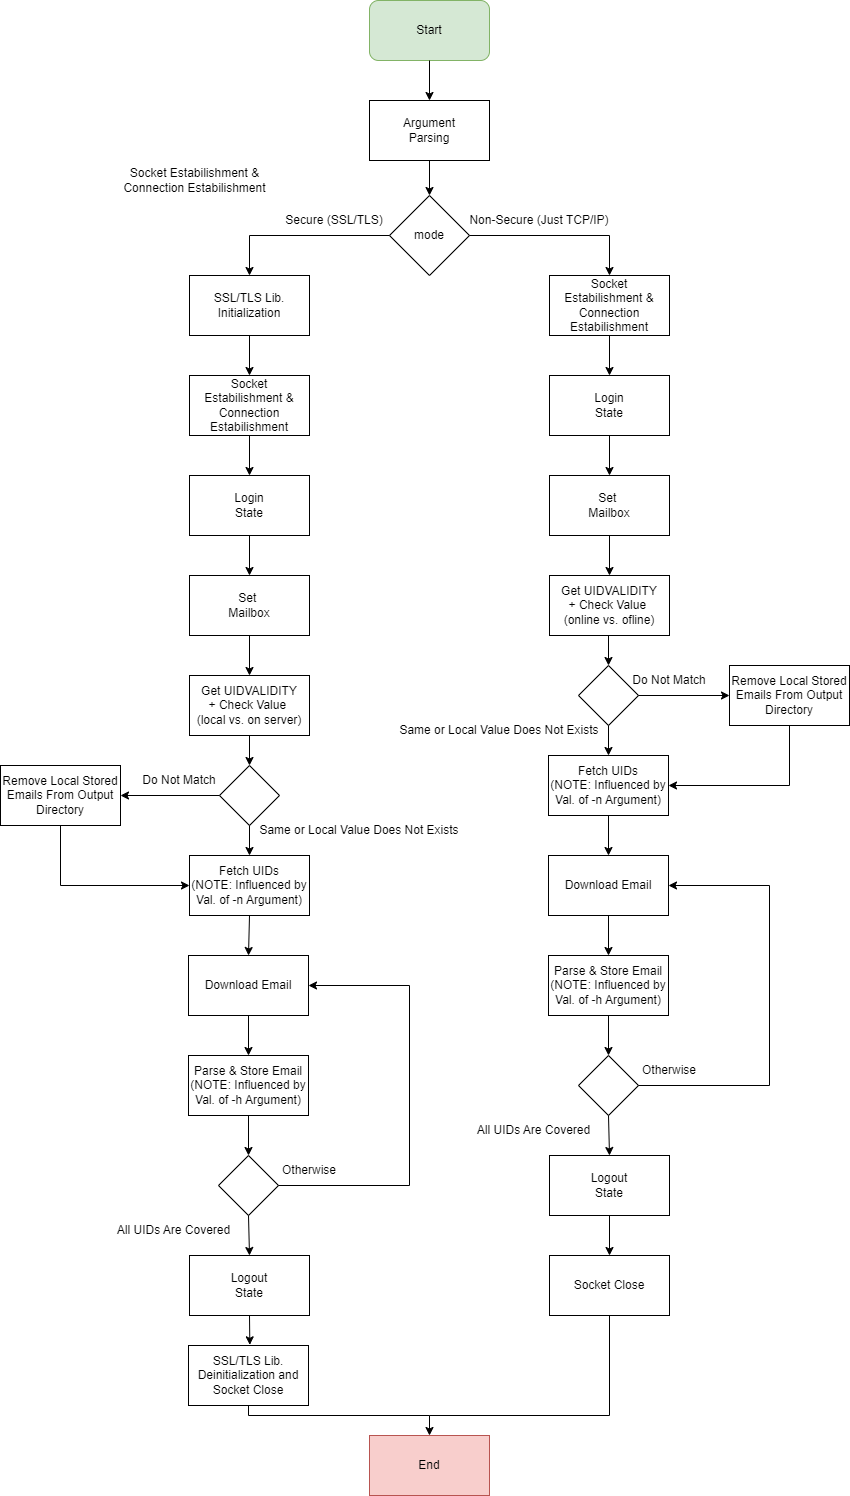
\includegraphics{program-flow-diagram.eps}
    }
    \caption{Program Flow Diagram}
    \label{figure:program-flow-diagram}
\end{figure}

\newpage
\subsection{Classes}
This section contains a visualization of the main program classes using a diagram based on 
the use-case diagram. The aim of these diagrams was to capture the individual classes and the 
methods/operations they allow.

\subsubsection{ClientConfig}
A class for processing user arguments, which is also responsible for storing the configuration 
of the future IMAP Client.

\begin{figure}[H]
    \centering
    \scalebox{0.5}{
        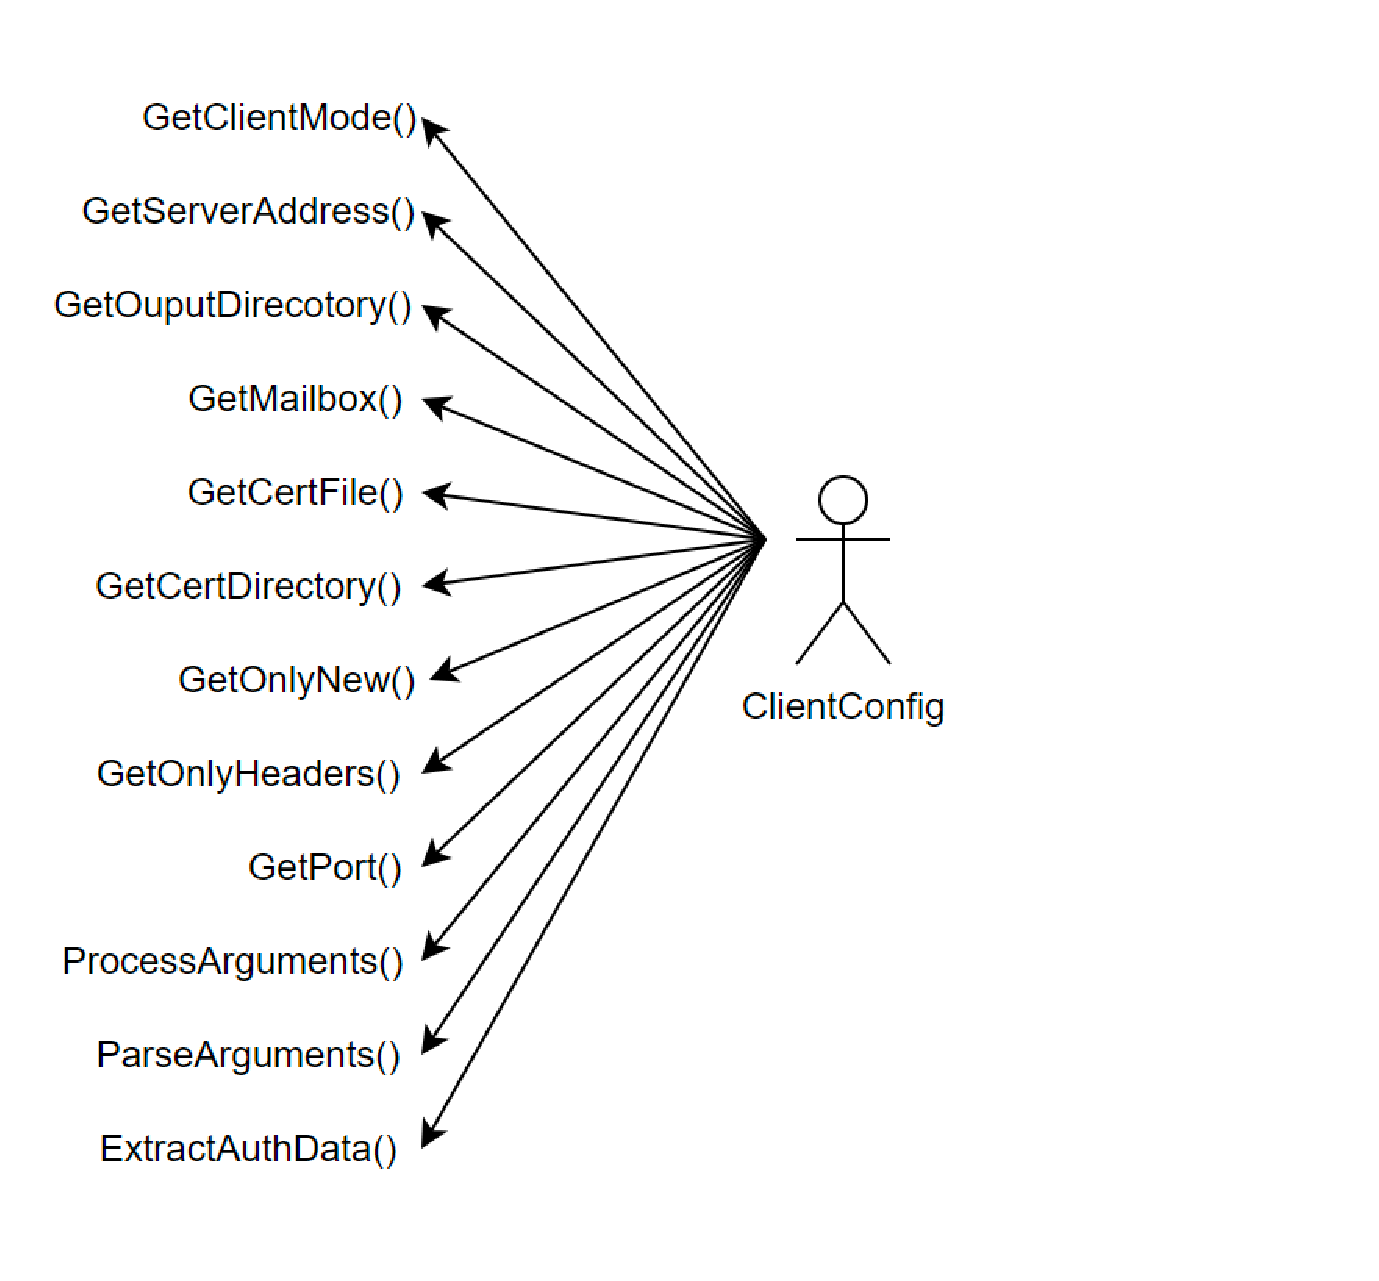
\includegraphics{ClientConfig.eps}
    }
    \caption{Class ClientConfig and ClientConfig Methods}
    \label{figure:client-config}
\end{figure}

\newpage

\subsubsection{ImapClients}
Here it may be seen that both \verb!SecureImapClient! and \verb!NonSecureImapClient! 
have a common ancestor, which is \verb!BaseImapClient! - providing common methods for 
both successors. On the basis of the configuration, an instance of the \verb!SecureImapClient! 
or \verb!NonSecureImapClient! class is created, it is responsible for taking care of 
the whole process of communication with the IMAP server and storing the results.

\begin{figure}[H]
    \centering
    \scalebox{0.3}{
        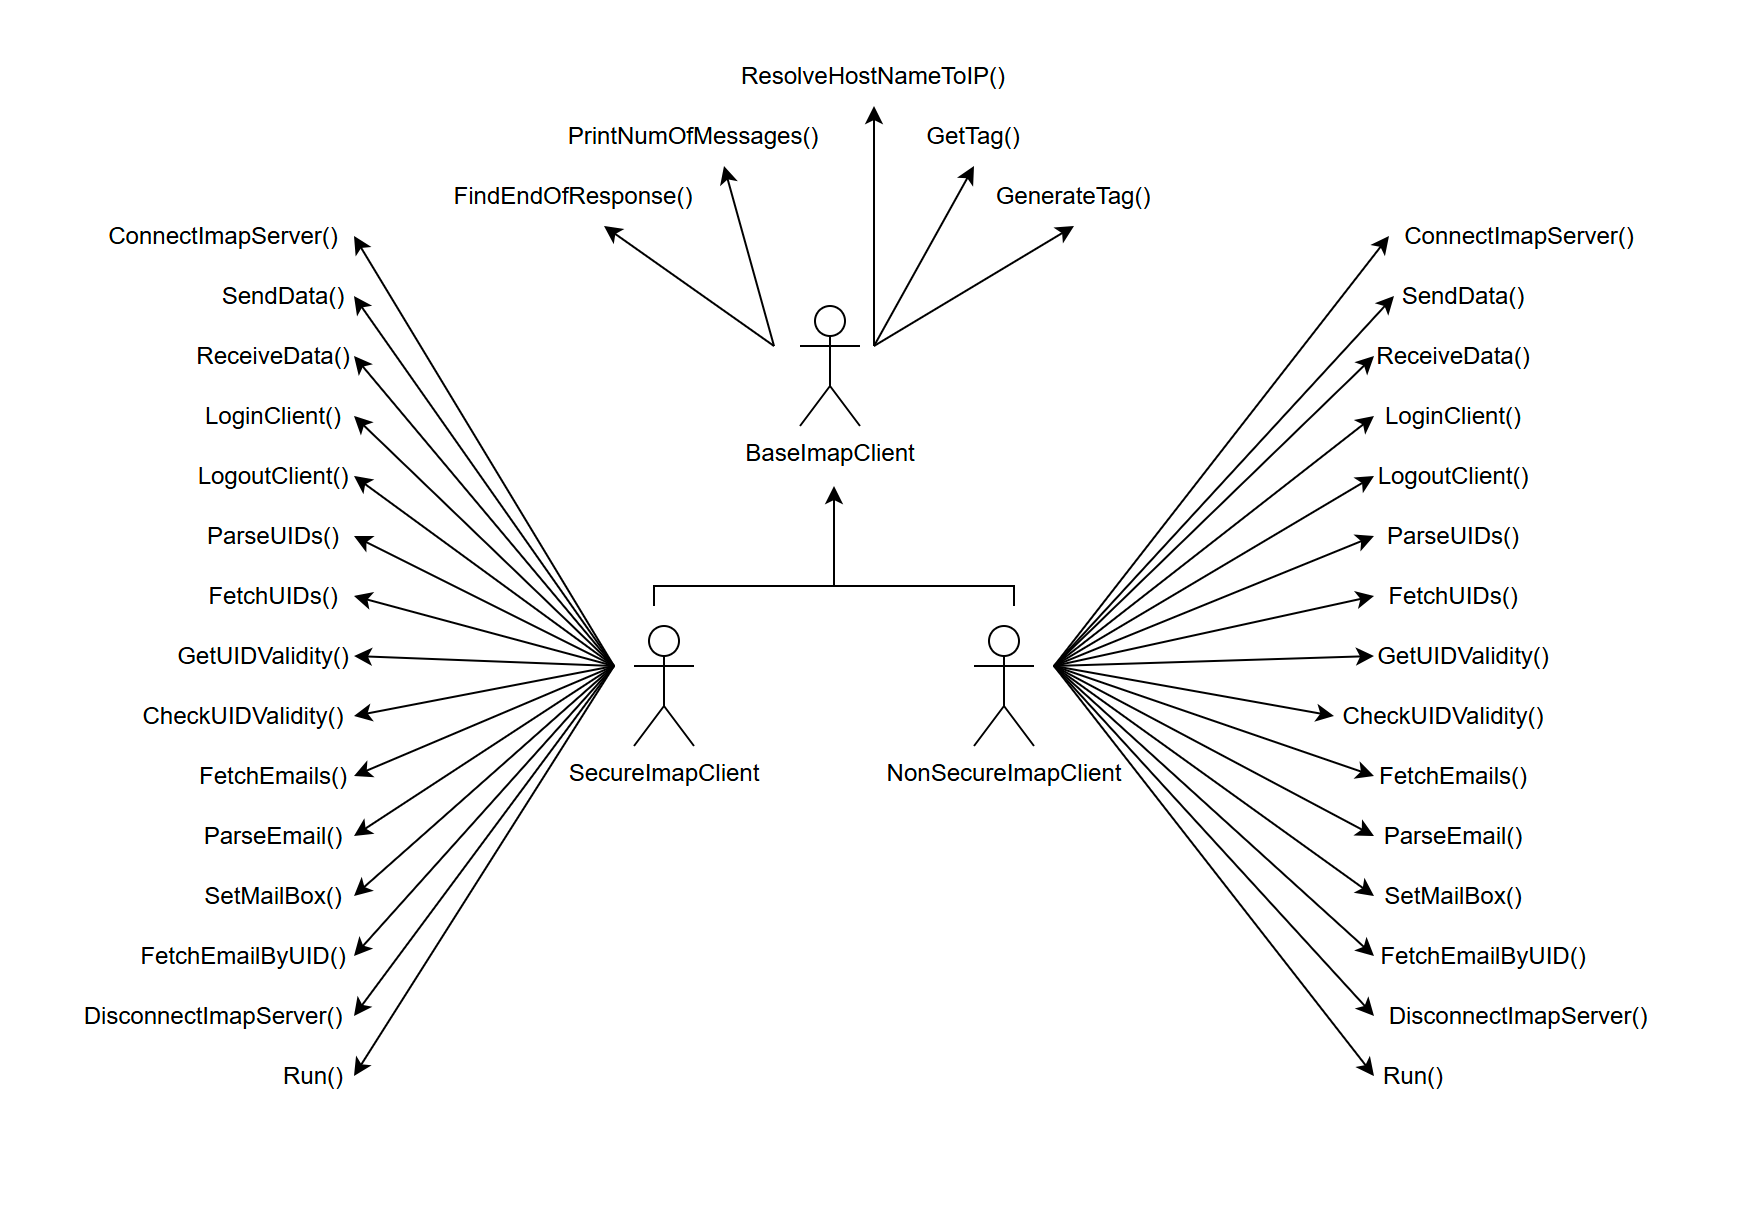
\includegraphics{ImapClient.eps}
    }
    \caption{ImapClient's Classes and Methods}
    \label{figure:imap-clients}
\end{figure}

\section{Testing}
The \verb!imapcl! program has also been tested. The testing was performed in two ways, 
the first one was tested using the local implementation of the IMAP server, the second 
way was chosen to test on foreign IMAP servers provided by the school such as eva or merlin.

\newpage

\subsection{Testing on Local IMAP Server}
To ensure the correct operation of the program, \texttt{imapcl} was tested using a local 
implementation of the IMAP server. The local IMAP server is available in the repository 
in the tests folder under the name \texttt{imap\_server.py}. The server is implemented in Python 
using the \texttt{os}, \texttt{socket}, \texttt{threading}, \texttt{subprocess}, 
\texttt{time}, and \texttt{signal} libraries and handles all requests from the client 
implementation such as \texttt{LOGIN}, \texttt{FETCH} (fetch support involves responding to 
specific requests such as \texttt{'tag' UID 'x' FETCH BODY[HEADER]} or \texttt{'tag' UID 'x' FETCH BODY[TEXT]} 
where \texttt{'tag'} is specific tag of the request and \texttt{'x'} is UID of the email), 
\texttt{SELECT}, and \texttt{LOGOUT}.

The tests folder also contains the test\_emails folder with sample emails that are sent to 
the IMAP client, at the same time these emails are used to compare what was sent with what 
was received on the IMAP client, the contents should be the same - the result of the 
comparison is displayed in the output of the script \texttt{imap\_server.py}.

The local IMAP server was used for basic testing of the application functionality, 
and at a later stage of development it was used to simulate errors and unusual conditions 
that can occur during communication between client and server.

\subsubsection{Implementation Details of Local IMAP Server}
To run the test correctly it is necessary to configure the parameters client\_path (containing the name of the binary file with the program), 
output\_dir (where the output files will be stored) and client\_args (arguments with which the tested program will be called), 
the local IMAP server uses the address 127.0.0.1 and runs by default on port 8143.

Here can we be seen the output of the test, which ended with success, 
the test during its run logs to the terminal information about what is currently happening.

\begin{figure}[H]
    \centering
    \scalebox{0.15}{
        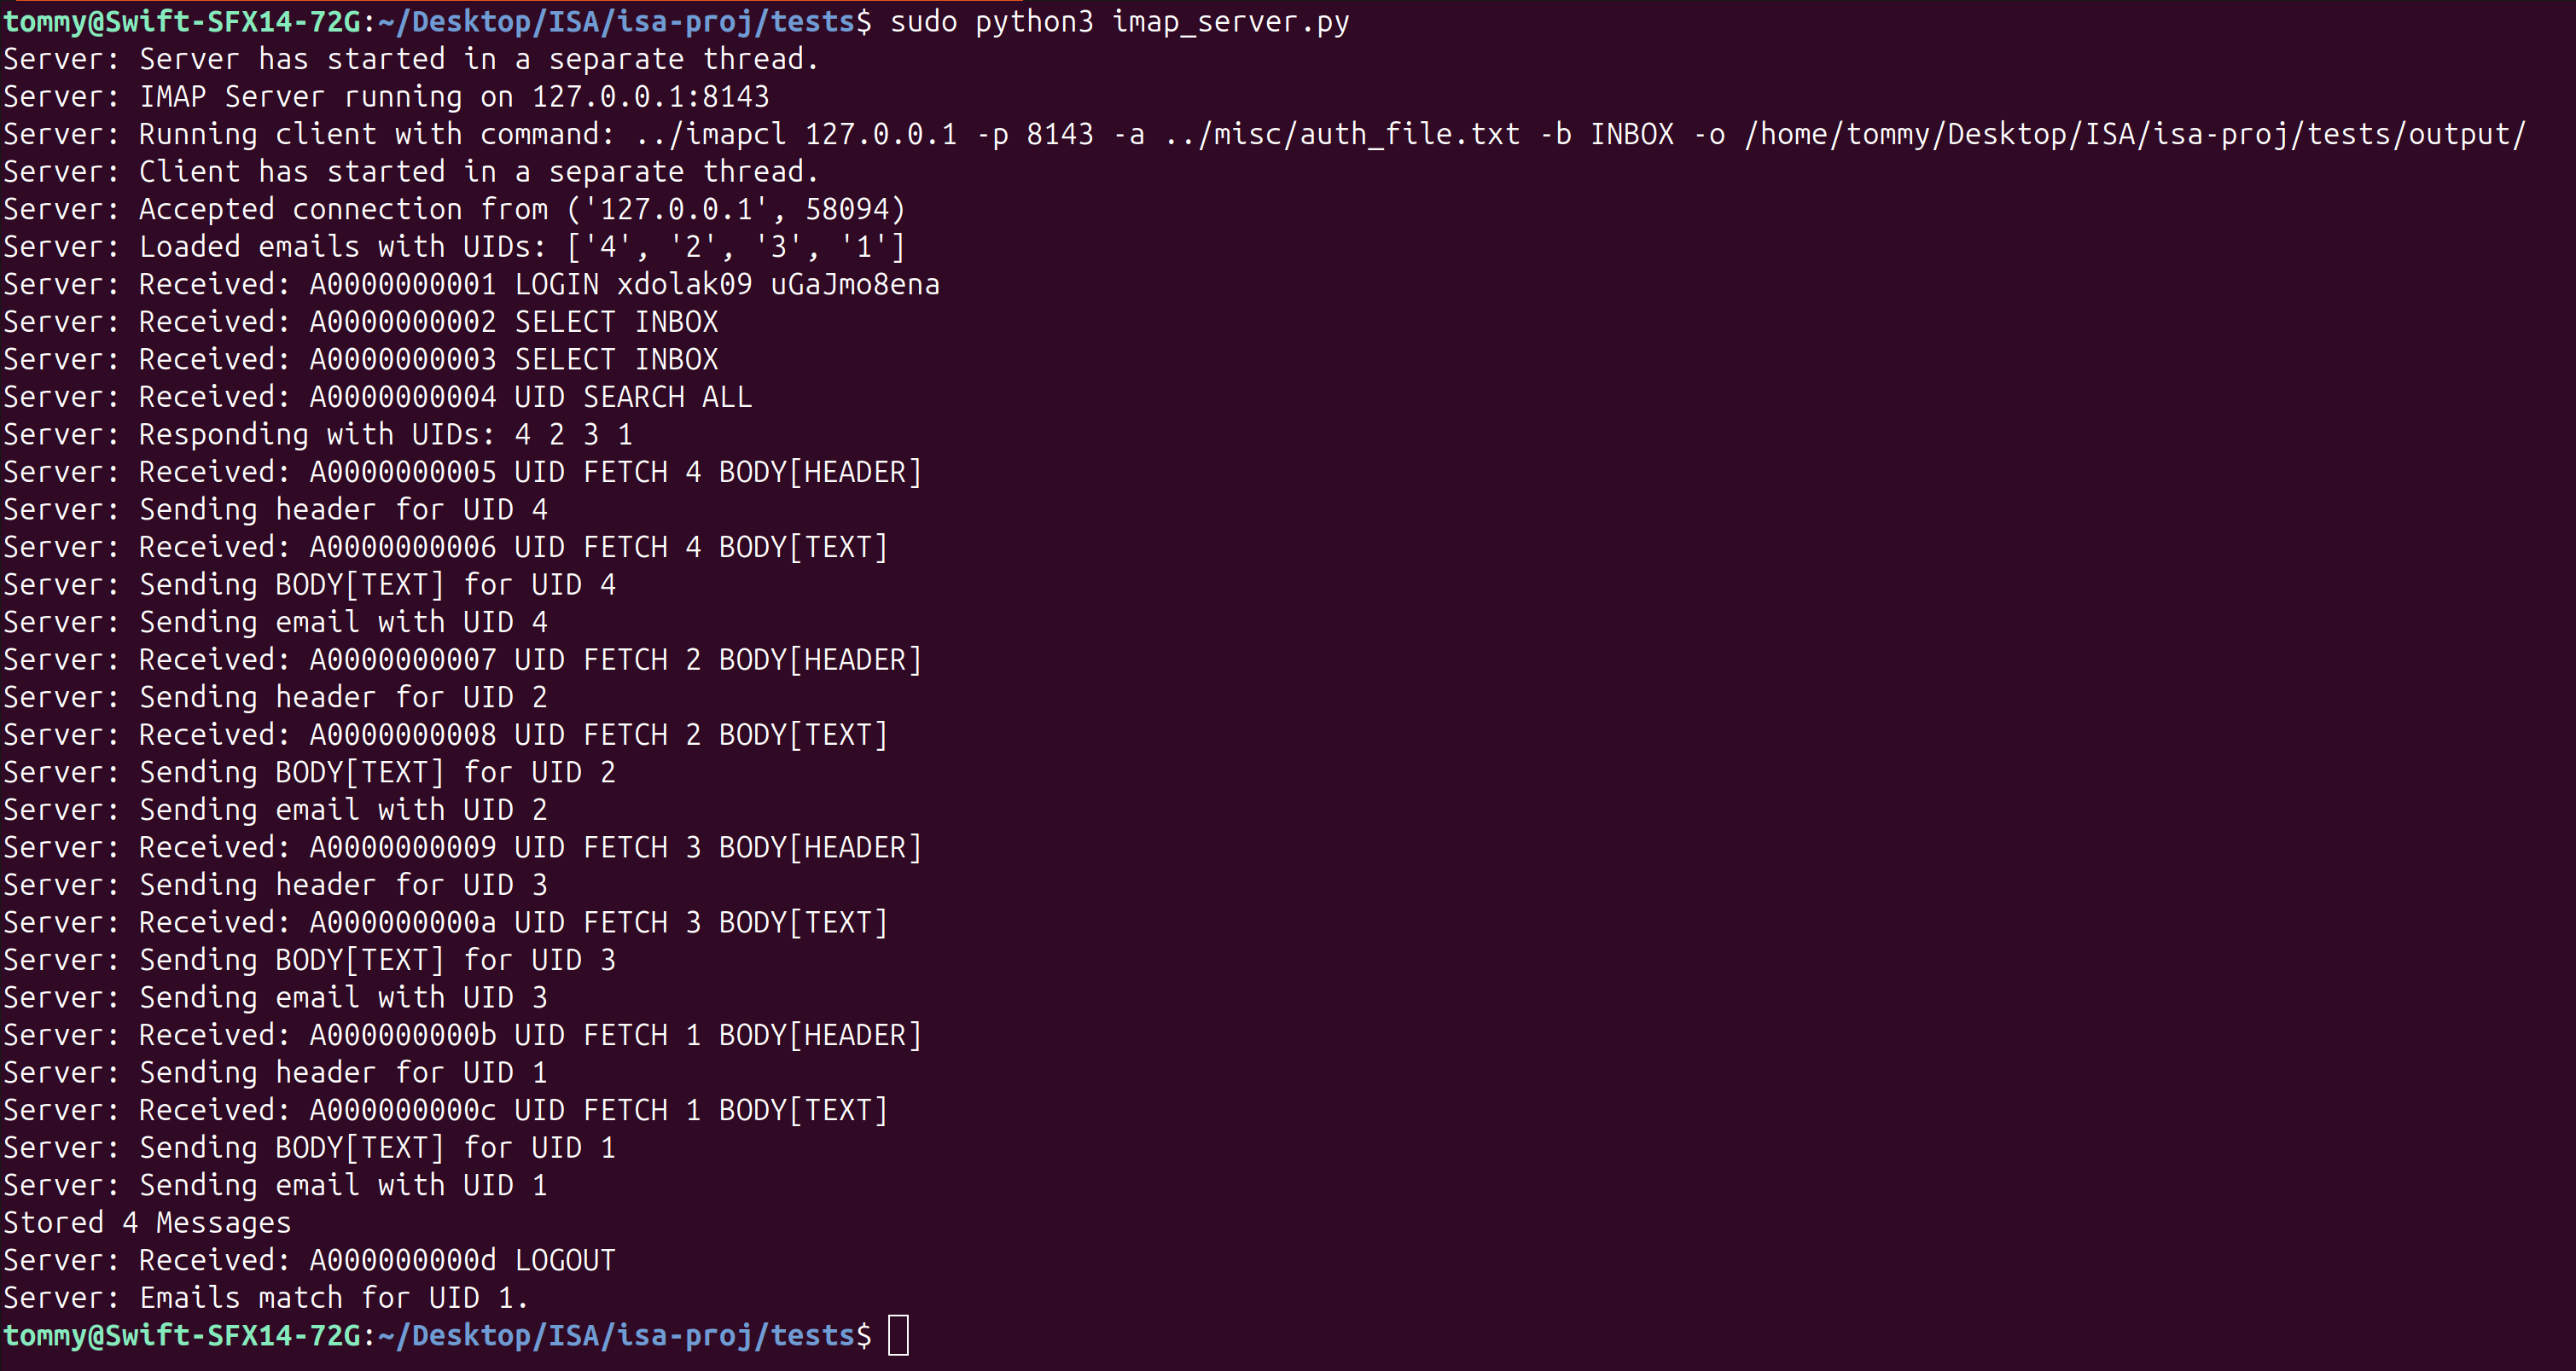
\includegraphics{imap_server.eps}
    }
    \caption{Output of imap\_server.py}
    \label{figure:imap-server}
\end{figure}

\begin{center}
    \vspace{0.5cm} % Space before table
    \begin{tabularx}{\textwidth}{|>{\raggedright\arraybackslash}p{5cm}|>{\raggedright\arraybackslash}p{5cm}|>{\raggedright\arraybackslash}X|}
        \hline
        \textbf{Testcase} & \textbf{Expected Output} & \textbf{Program Output} \\
        \hline
        Server does not responds to \texttt{LOGIN} command. & Program should exit with \texttt{BAD\_RESPONSE} error code. & Program ends with \texttt{BAD\_RESPONSE} error code. \\
        \hline
        Server sends different end of response string (e.g. not \texttt{TAG OK FETCH Completed} but \texttt{TAG OK fetch}). & Client should handle this kind change and continue. & Client successfully proceeds and completes its download. \\
        \hline
        Server sends different \texttt{.uidvalidity} value for mailbox. & Output directory should be cleared and emails should be downloaded again. & Output directory is cleared and emails are downloaded again. \\
        \hline
        Server does not respond at all. & Client should successfully end and print error message on stderr. & Client successfully ends and prints error message on stderr.  \\
        \hline
        Stress test, sending three emails, size of each of them 33MB. & Emails successfully downloaded. & Emails were successfully downloaded. Note: Speed was not optimal. \\
        \hline
        Sent an email whose size slightly exceeds the receiving buffer (the end of the email is split into two parts) & No freezing of the program and email successfully downloaded. & No freezing of the program and email successfully downloaded. \\
        \hline
    \end{tabularx}
    \vspace{0.5cm} % Space after table
\end{center}

\subsection{Testing on Foreign IMAP Servers}
As a complementary method, testing on foreign IMAP servers provided by the school, such as eva 
or merlin, was chosen to ensure compatibility outside the local environment and to demonstrate 
the usability of the program.

\begin{center}
    \vspace{0.5cm} % Space before table
    \begin{tabularx}{\textwidth}{|>{\raggedright\arraybackslash}p{5cm}|>{\raggedright\arraybackslash}p{1cm}|>{\raggedright\arraybackslash}p{5cm}|>{\raggedright\arraybackslash}X|}
        \hline
        \textbf{Testcase} & \textbf{Server} & \textbf{Expected Output} & \textbf{Program Output} \\
        \hline
        Compilation & eva & Successful compilation. & Successful compilation. \\
        \hline
        Auth. file parsing & eva & Auth. file successfully parsed & Auth. file successfully parsed. \\
        \hline
        Calling \texttt{./imapcl outlook.office365.com -p 143 -a PATH/auth\_file.txt -b INBOX -o PATH/output/} & eva & Downloaded whole emails (including header and body), note: number emails on server was 1739. & Downloaded 1739 from server with headers and bodies. \\
        \hline
        Calling \texttt{./imapcl outlook.office365.com -p 143 -a PATH/auth\_file.txt -b INBOX -o PATH/output/} with changed value of \texttt{.uidvalidity} file & eva & Downloaded whole emails (including header and body) and updated value in \texttt{.uidvalidity} file, note: number emails on server was 1739 & Downloaded 1739 from server with headers and bodies. Updated valued of \texttt{.uidvalidity} file. \\
        \hline
    \end{tabularx}
    \vspace{0.5cm} % Space after table
\end{center}

\begin{center}
    \vspace{0.5cm} % Space before table
    \begin{tabularx}{\textwidth}{|>{\raggedright\arraybackslash}p{5cm}|>{\raggedright\arraybackslash}p{1cm}|>{\raggedright\arraybackslash}p{5cm}|>{\raggedright\arraybackslash}X|}
        \hline
        \textbf{Testcase} & \textbf{Server} & \textbf{Expected Output} & \textbf{Program Output} \\
        \hline
        Calling \texttt{./imapcl outlook.office365.com -p 143 -a PATH/auth\_file.txt -b INBOX -o PATH/output/} and path \texttt{PATH/output/} does not exists & eva & Downloaded whole emails (including header and body) and created output directory in \texttt{PATH/output/} file, note: number emails on server was 1739 & Downloaded 1739 from server with headers and bodies. in output directory \texttt{PATH/output/}. \\
        \hline
        Calling \texttt{./imapcl outlook.office365.com -T -a PATH/auth\_file.txt -b INBOX -o PATH/output/} with changed value of \texttt{.uidvalidity} file & eva & Downloaded whole emails (including header and body) and updated value in \texttt{.uidvalidity} file thru SSL/TLS on port 993, note: number emails on server was 1739 & Downloaded 1739 from server with headers and bodies. Updated valued of \texttt{.uidvalidity} file. Used SSL/TLS on default port 993.\\
        \hline
        Compilation & merlin & Successful Compilation & Successful Compilation \\
        \hline
        Auth. file parsing & merlin & Auth. file successfully parsed & Auth. file successfully parsed. \\
        \hline
        Calling \texttt{./imapcl eva.fit.vutbr.cz -p 143 -a PATH/auth\_file.txt -b INBOX -o PATH/output/} & merlin & Downloaded whole emails (including header and body), note: number emails on server was 2349. & Downloaded 2349 from server with headers and bodies. \\
        \hline
        Calling \texttt{./imapcl eva.fit.vutbr.cz -p 143 -h -a PATH/auth\_file.txt -b INBOX -o PATH/output/} & merlin & Downloaded email only headers, note: number emails on server was 2349. & Downloaded 2349 email headers from server. \\
        \hline
        Calling \texttt{./imapcl eva.fit.vutbr.cz -p 143 -n -a PATH/auth\_file.txt -b INBOX -o PATH/output/} & merlin & Downloaded email only new emails (headers + bodies), note: number emails on server was 56. & Downloaded 56 new emails from server with headers and bodies. \\
        \hline
        Calling \texttt{./imapcl eva.fit.vutbr.cz -p 143 -n -a PATH/auth\_file.txt -b BOX1 -o PATH/output/} & merlin & Two emails should be downloaded and \texttt{UIDVALIDITY} of \texttt{BOX1} should be stored into \texttt{.uidvalidity.txt} & Two emails were downloaded and \texttt{UIDVALIDITY} of \texttt{BOX1} were saved into \texttt{.uidvalidity.txt} \\
        \hline
        Calling \texttt{./imapcl eva.fit.vutbr.cz -T -p 993 -n -a PATH/auth\_file.txt -b INBOX -o PATH/output/} & merlin & For SSL cetificates should be used default location - \texttt{/etc/ssl/certs}. & Used default location for SSL certificates, \texttt{/etc/ssl/certs}. \\
        \hline
    \end{tabularx}
    \vspace{0.5cm} % Space after table
\end{center}

\begin{center}
    \vspace{0.5cm} % Space before table
    \begin{tabularx}{\textwidth}{|>{\raggedright\arraybackslash}p{5cm}|>{\raggedright\arraybackslash}p{1cm}|>{\raggedright\arraybackslash}p{5cm}|>{\raggedright\arraybackslash}X|}
        \hline
        \textbf{Testcase} & \textbf{Server} & \textbf{Expected Output} & \textbf{Program Output} \\
        \hline
        Calling \texttt{./imapcl eva.fit.vutbr.cz -T -p 993 -n -a PATH/auth\_file.txt -b BOX1 -o PATH/output/} with stored all emails from mailbox and right value of \texttt{UIDVALIDITY} & merlin & Zero emails should be downloaded & Zero emails downloaded. \\
        \hline
        Calling \texttt{./imapcl eva.fit.vutbr.cz -p 143 -h -n -a PATH/auth\_file.txt -b INBOX -o PATH/output/} & merlin & Downloaded email only new emails (only headers), note: number emails on server was 56. & Downloaded 56 headers of new emails from server. \\
        \hline
        Calling \texttt{./imapcl eva.fit.vutbr.cz -g 143 -h -n -a PATH/auth\_file.txt -b INBOX -o PATH/output/} & merlin & Wrong argument \texttt{-g}, help on terminal should be printed. & Printed help to the user on terminal. \\
        \hline
        Calling \texttt{./imapcl eva.fit.vutbr.cz -p 143} & merlin & A small number of arguments for calling the program. The error message should be displayed to the user. & Displayed the error message that informs user a small number of arguments for calling the program that were used.\\
        \hline
    \end{tabularx}
    \vspace{0.5cm} % Space after table
\end{center}

\section{Return Codes}
The program is designed in such a way that in case of an error or failure, the user 
is always informed about the situation that has occurred. In case of success the program 
always returns the return value 0 (respectively \verb!SUCCESS!), in other cases the program gives the return 
values according to the table below.

\begin{center}
    \vspace{0.5cm} % % Space before table
    \begin{tabularx}{\textwidth}{|>{\raggedright\arraybackslash}p{6.5cm}|>{\raggedright\arraybackslash}p{2cm}|>{\raggedright\arraybackslash}p{1.5cm}|>{\raggedright\arraybackslash}X|}
        \hline
        \textbf{Name} & \textbf{Data Type} & \textbf{Value} & \textbf{Description} \\
        \hline
        OUTPUT\_DIR\_NOT\_CREATED & int & -7 & Output Directory Could Not Be Created \\
        \hline
        UIDVALIDITY\_FILE\_NOT\_FOUND & int & -6 & .uidvalidity File Not Found \\
        \hline
        UIDVALIDITY\_FILE\_ERROR & int & -5 & Error With .uidvalidity File (Invalid Format, Out of Range) \\
        \hline
        CREATE\_CONNECTION\_FAILED & int & -4 & Failed to Create Connection With IMAP Server \\
        \hline
        SSL\_CERT\_VERIFICATION\_FAILED & int & -3 & SSL Certificate Verification Failed \\
        \hline
    \end{tabularx}
    \vspace{0.5cm} % Space after table
\end{center}

\begin{center}
    \vspace{0.5cm} % % Space before table
    \begin{tabularx}{\textwidth}{|>{\raggedright\arraybackslash}p{6.5cm}|>{\raggedright\arraybackslash}p{2cm}|>{\raggedright\arraybackslash}p{1.5cm}|>{\raggedright\arraybackslash}X|}
        \hline
        FETCH\_EMAIL\_FAILED & int & -2 & Fetching Email By UID Failed \\
        \hline
        SUCCESS & int & 0 & Operation Was Successful \\
        \hline
        NO\_IP\_ADDR\_FOUND & int & 1 & No IPv4 Address Was Found \\
        \hline
        PARSE\_ARGUMENTS\_FAILED & int & 2 & Parsing Program's Arguments Failed \\
        \hline
        PARSE\_CREDENTIALS\_FAILED & int & 3 & Parsing Credentials Failed \\
        \hline
        SERVER\_UNKNOWN\_RESPONSE & int & 4 & Server Sent an Unknown Response \\
        \hline
        TRANSMIT\_DATA\_FAILED & int & 5 & Transmission of Data Failed \\
        \hline
        RECEIVE\_DATA\_FAILED & int & 6 & Reception of Data Failed \\
        \hline
        RESPONSE\_NOT\_FOUND & int & 7 & Expected Server's Response Was Not Found \\
        \hline
        PARSE\_BY\_REGEX\_FAILED & int & 8 & Parsing of Regular Expression Failed \\
        \hline
        NON\_UIDS\_RECEIVED & int & 9 & No UIDs Were Received From The IMAP Server \\
        \hline
        CONTINUE\_IN\_RECEIVING & int & 10 & Continue Receiving More Data \\
        \hline
        UNDEFINED\_STATE & int & 11 & Undefined State Encountered \\
        \hline
        UID\_VALIDITY\_ERROR\_IN\_RECV & int & 14 & Unable to Receive UIDVALIDITY From The Server \\
        \hline
        REMOVAL\_OF\_EMAILS\_FAILED & int & 15 & Failed to Remove Emails When UIDVALIDITY Does Not Match \\
        \hline
        BAD\_RESPONSE & string & "Bad Response :(" & Error During Receiving of Server's Response \\
        \hline
    \end{tabularx}
    \vspace{0.5cm} % Space after table
\end{center}

\newpage

\bibliographystyle{unsrt}
\bibliography{resources}      
\end{document}